\chapter{HASIL DAN PEMBAHASAN}
Pada penelitian ini dipaparkan hasil penelitian serta analisis dari model klasifikasi yang telah dibuat sesuai dengan desain sistem dan implementasi pada Bab 3. Data yang digunakan pada pengujian ini menggunakan dataset DRAC dengan data splitting yang telah dilakukan pra-pemrosesan sebelumnya.
\section{Hasil Penelitian}

\section{Hasil Pengujian}
\subsection{Hasil pengujian Model tanpa menggunakan penyesuaian apapun}

    \begin{table}[H]
        \begin{center}
        \caption{Hasil training best model tanpa melalui penyesuaian class dataset}
        \label{tb:HasilTrainClassWeight}
            \begin{tabular}{clclll}
            \cline{1-6}
            ResNet   architecture & \multicolumn{1}{c}{class} & acc                     & \multicolumn{1}{c}{prec} & \multicolumn{1}{c}{rec} & \multicolumn{1}{c}{F1} \\ \cline{1-6}
            \multirow{3}{*}{18}   & non-DR                    & \multirow{3}{*}{0,7642} & 0,861538                 & 0,848485                & 0,854962               \\
                                  & NPDR                      &                         & 0,652174                 & 0,697674                & 0,674157               \\
                                  & PDR                       &                         & 0,666667                 & 0,571429                & 0,615385               \\ \cline{1-6}
            \multirow{3}{*}{34}   & non-DR                    & \multirow{3}{*}{0,7724} & 0,857143                 & 0,818182                & 0,837209               \\
                                  & NPDR                      &                         & 0,666667                 & 0,790698                & 0,723404               \\
                                  & PDR                       &                         & 0,777778                 & 0,5                     & 0,608696               \\ \cline{1-6}
            \multirow{3}{*}{50}   & non-DR                    & \multirow{3}{*}{0,6992} & 0,808824                 & 0,833333                & 0,820896               \\
                                  & NPDR                      &                         & 0,581395                 & 0,581395                & 0,581395               \\
                                  & PDR                       &                         & 0,5                      & 0,428571                & 0,461538               \\ \cline{1-6}
            \multirow{3}{*}{101}  & non-DR                    & \multirow{3}{*}{0,8049} & 0,909091                 & 0,909091                & 0,909091               \\
                                  & NPDR                      &                         & 0,711111                 & 0,744186                & 0,727273               \\ 
                                  & PDR                       &                         & 0,583333                 & 0,5                     & 0,538462               \\ \cline{1-6}
            \multirow{3}{*}{152}  & non-DR                    & \multirow{3}{*}{0,7398} & 0,852459                 & 0,787879                & 0,818898               \\
                                  & NPDR                      &                         & 0,603774                 & 0,744186                & 0,666667               \\
                                  & PDR                       &                         & 0,777778                 & 0,5                     & 0,608696               \\ \cline{1-6}
            \end{tabular}
        \end{center}
    \end{table}


\subsection{Hasil Pengujian Model dengan penyesuaian menggunakan class-weight}

    \begin{figure}[H]
        \centering
        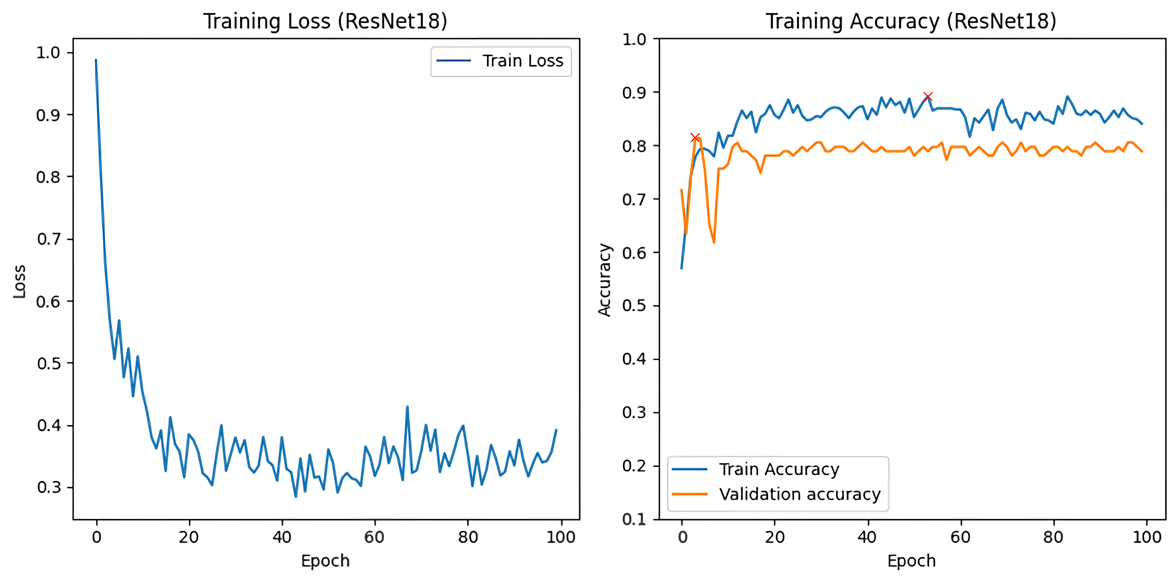
\includegraphics[scale=0.8]{gambar/TrainingGraphResNet18class-weighted.png}
        \caption{Training Loss dan Akurasi ResNet-18}
        \label{Img:GraphResNet18}
    \end{figure}
    \begin{figure}[H]
        \centering[width=\textwidth]
        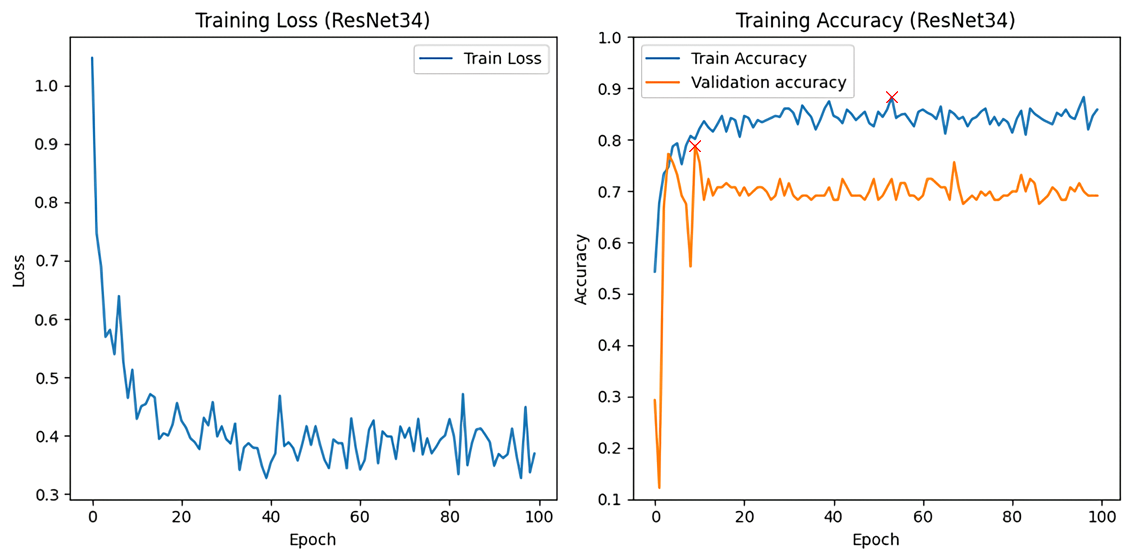
\includegraphics[scale=0.85]{gambar/TrainingGraphResNet34class-weighted.png}
        \caption{Training Loss dan Akurasi ResNet-34}
        \label{Img:GraphResNet34}
    \end{figure}
    \begin{figure}[H]
        \centering
        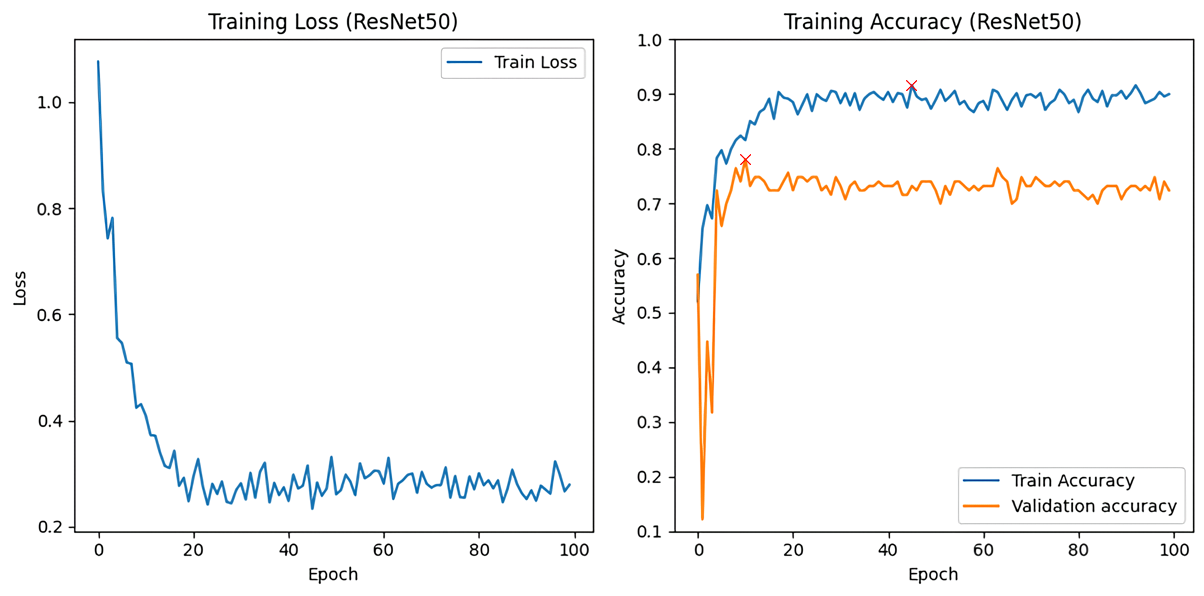
\includegraphics[scale=0.8]{gambar/TrainingGraphResNet50class-weighted.png}
        \caption{Training Loss dan Akurasi ResNet-50}
        \label{Img:GraphResNet50}
    \end{figure}
    \begin{figure}[]
        \centering
        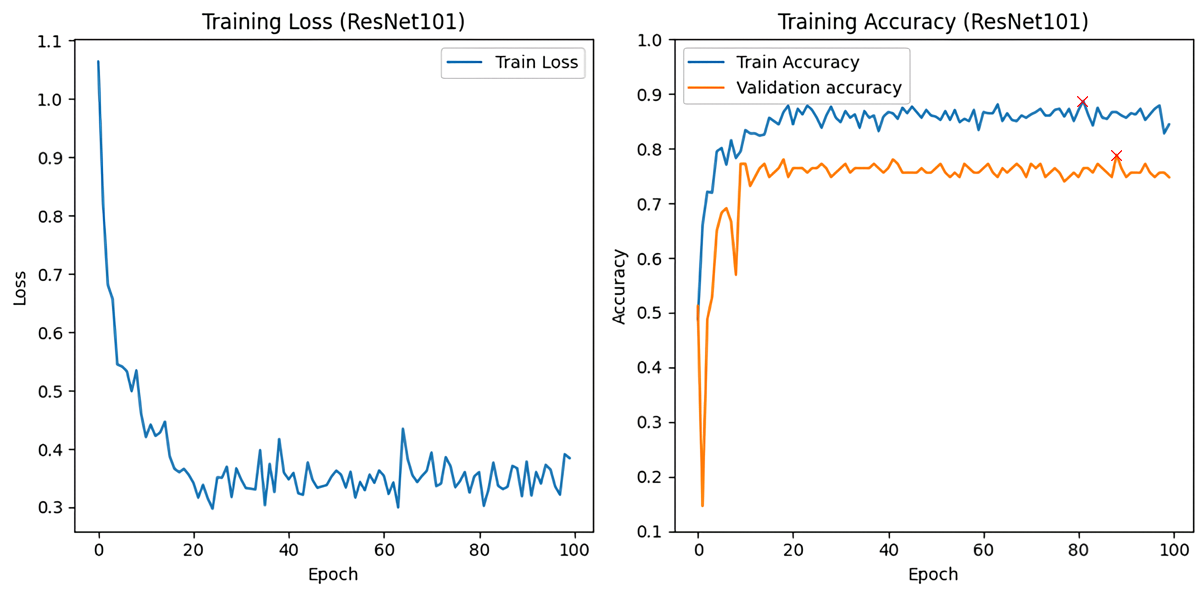
\includegraphics[scale=0.8]{gambar/TrainingGraphResNet101class-weighted.png}
        \caption{Training Loss dan Akurasi ResNet-101}
        \label{Img:GraphResNet101}
    \end{figure}
    \begin{figure}
        \centering
        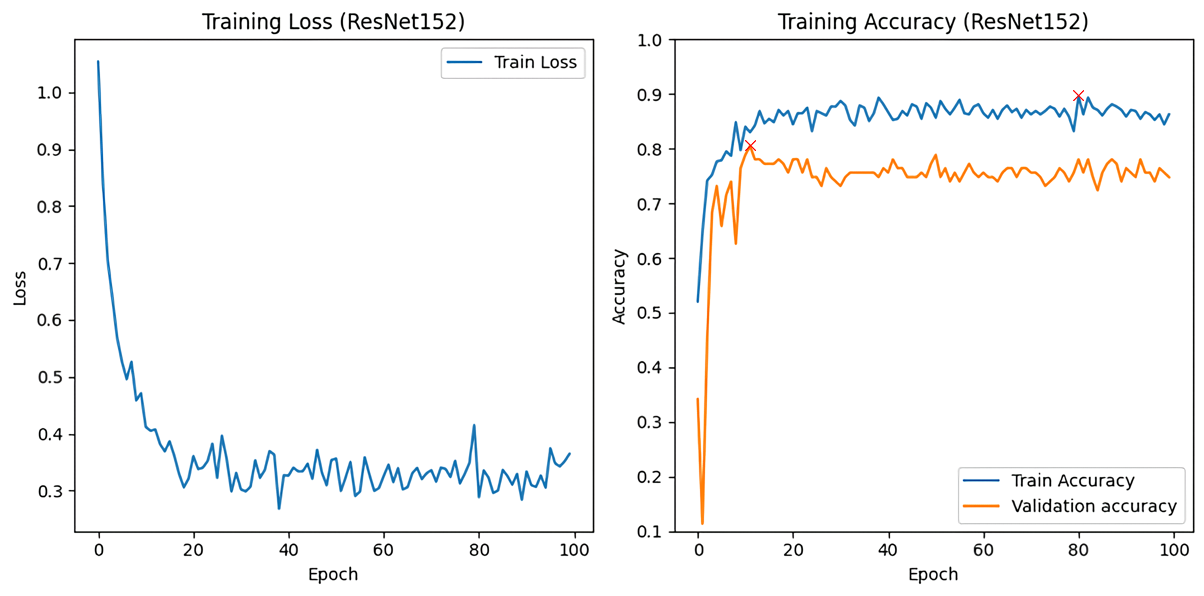
\includegraphics[scale=0.8]{gambar/TrainingGraphResNet152class-weighted.png}
        \caption{Training Loss dan Akurasi ResNet-152}
        \label{Img:GraphResNet152}
    \end{figure}


    \begin{table}[h!]
        \begin{center}
        \caption{Hasil best trained model menggunakan class-weight adjustment}
        \label{tb:HasilTrainClassWeight}
            \begin{tabular}{|c|l|c|l|l|l|c|}
            \hline
            ResNet   architecture & \multicolumn{1}{c|}{class} & acc                     & \multicolumn{1}{c|}{prec} & \multicolumn{1}{c|}{rec} & \multicolumn{1}{c|}{F1} & QWK                                 \\ \hline
            \multirow{3}{*}{18}   & non-DR                     & \multirow{3}{*}{0,7886} & 0,875                     & 0,848485                 & 0,861538                & \multirow{3}{*}{0.7526956474324895} \\ \cline{2-2} \cline{4-6}
                                  & NPDR                       &                         & 0,704545                  & 0,72093                  & 0,712644                &                                     \\ \cline{2-2} \cline{4-6}
                                  & PDR                        &                         & 0,666667                  & 0,714286                 & 0,689655                &                                     \\ \hline
            \multirow{3}{*}{34}   & non-DR                     & \multirow{3}{*}{0,7236} & 0,877193                  & 0,757576                 & 0,813008                & \multirow{3}{*}{0.7344195070936137} \\ \cline{2-2} \cline{4-6}
                                  & NPDR                       &                         & 0,617021                  & 0,674419                 & 0,644444                &                                     \\ \cline{2-2} \cline{4-6}
                                  & PDR                        &                         & 0,526316                  & 0,714286                 & 0,606061                &                                     \\ \hline
            \multirow{3}{*}{50}   & non-DR                     & \multirow{3}{*}{0,7317} & 0,848485                  & 0,848485                 & 0,848485                & \multirow{3}{*}{0.7416221605070141} \\ \cline{2-2} \cline{4-6}
                                  & NPDR                       &                         & 0,634146                  & 0,604651                 & 0,619048                &                                     \\ \cline{2-2} \cline{4-6}
                                  & PDR                        &                         & 0,5                       & 0,571429                 & 0,533333                &                                     \\ \hline
            \multirow{3}{*}{101}  & non-DR                     & \multirow{3}{*}{0,7642} & 0,916667                  & 0,833333                 & 0,873016                & \multirow{3}{*}{0.7133252550521831} \\ \cline{2-2} \cline{4-6}
                                  & NPDR                       &                         & 0,666667                  & 0,651163                 & 0,658824                &                                     \\ \cline{2-2} \cline{4-6}
                                  & PDR                        &                         & 0,52381                   & 0,785714                 & 0,628571                &                                     \\ \hline
            \multirow{3}{*}{152}  & non-DR                     & \multirow{3}{*}{0,7805} & 0,870968                  & 0,818182                 & 0,84375                 & \multirow{3}{*}{0.7423939072743689} \\ \cline{2-2} \cline{4-6}
                                  & NPDR                       &                         & 0,714286                  & 0,697674                 & 0,705882                &                                     \\ \cline{2-2} \cline{4-6}
                                  & PDR                        &                         & 0,631579                  & 0,857143                 & 0,727273                &                                     \\ \hline
            \end{tabular}
        \end{center}
    \end{table}
    \begin{table}[h!]
        \begin{center}
        \caption{Hasil best validated model menggunakan class-weight adjustment}
        \label{tb:HasilValClassWeight}
            \begin{tabular}{|c|l|c|l|l|l|c|}
            \hline
            ResNet   architecture & \multicolumn{1}{c|}{class} & acc                     & \multicolumn{1}{c|}{prec} & \multicolumn{1}{c|}{rec} & \multicolumn{1}{c|}{F1} & QWK                                 \\ \hline
            \multirow{3}{*}{18}   & non-DR                     & \multirow{3}{*}{0,813}  & 0,869565                  & 0,909091                 & 0,888889                & \multirow{3}{*}{0.6266311390141076} \\ \cline{2-2} \cline{4-6}
                                  & NPDR                       &                         & 0,717391                  & 0,767442                 & 0,741573                &                                     \\ \cline{2-2} \cline{4-6}
                                  & PDR                        &                         & 0,875                     & 0,5                      & 0,636364                &                                     \\ \hline
            \multirow{3}{*}{34}   & non-DR                     & \multirow{3}{*}{0,7886} & 0,777778                  & 0,954545                 & 0,857143                & \multirow{3}{*}{0.6915275416648504} \\ \cline{2-2} \cline{4-6}
                                  & NPDR                       &                         & 0,88                      & 0,511628                 & 0,647059                &                                     \\ \cline{2-2} \cline{4-6}
                                  & PDR                        &                         & 0,705882                  & 0,857143                 & 0,774194                &                                     \\ \hline
            \multirow{3}{*}{50}   & non-DR                     & \multirow{3}{*}{0,7805} & 0,84058                   & 0,878788                 & 0,859259                & \multirow{3}{*}{0.7084479219119185} \\ \cline{2-2} \cline{4-6}
                                  & NPDR                       &                         & 0,690476                  & 0,674419                 & 0,682353                &                                     \\ \cline{2-2} \cline{4-6}
                                  & PDR                        &                         & 0,75                      & 0,642857                 & 0,692308                &                                     \\ \hline
            \multirow{3}{*}{101}  & non-DR                     & \multirow{3}{*}{0,7886} & 0,907692                  & 0,893939                 & 0,900763                & \multirow{3}{*}{0.7076588090504592} \\ \cline{2-2} \cline{4-6}
                                  & NPDR                       &                         & 0,72973                   & 0,627907                 & 0,675                   &                                     \\ \cline{2-2} \cline{4-6}
                                  & PDR                        &                         & 0,52381                   & 0,785714                 & 0,628571                &                                     \\ \hline
            \multirow{3}{*}{152}  & non-DR                     & \multirow{3}{*}{0,8049} & 0,870968                  & 0,818182                 & 0,84375                 & \multirow{3}{*}{0.7052973650209466} \\ \cline{2-2} \cline{4-6}
                                  & NPDR                       &                         & 0,733333                  & 0,767442                 & 0,75                    &                                     \\ \cline{2-2} \cline{4-6}
                                  & PDR                        &                         & 0,75                      & 0,857143                 & 0,8                     &                                     \\ \hline
            \end{tabular}
        \end{center}
    \end{table}
    
    \begin{figure}[H]
        \begin{minipage}[t]{0.475\textwidth} %d
            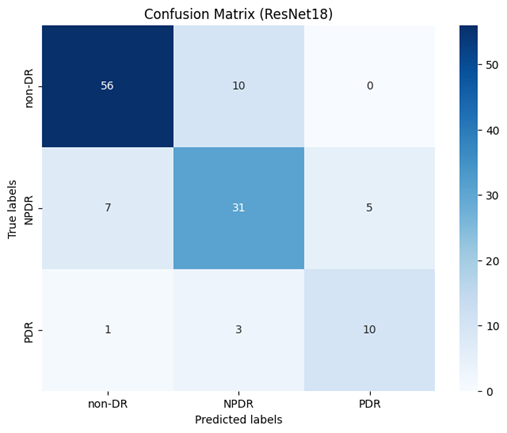
\includegraphics[draft=false, width=\textwidth]{gambar/confusionMatrixResnet18class-weighted_bestTrain.png} 
            \caption{Image A}
            \label{fig:1a}
        \end{minipage}
        \hfill
        \begin{minipage}[t]{0.475\textwidth} %
            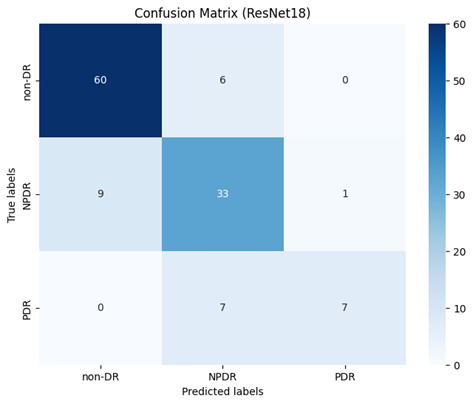
\includegraphics[draft=false, width=\textwidth]{gambar/confusionMatrixResnet18class-weighted_bestVal.png} 
            \caption{Image D}
            \label{fig:2b}
        \end{minipage}
        \begin{minipage}[t]{0.475\textwidth} %
            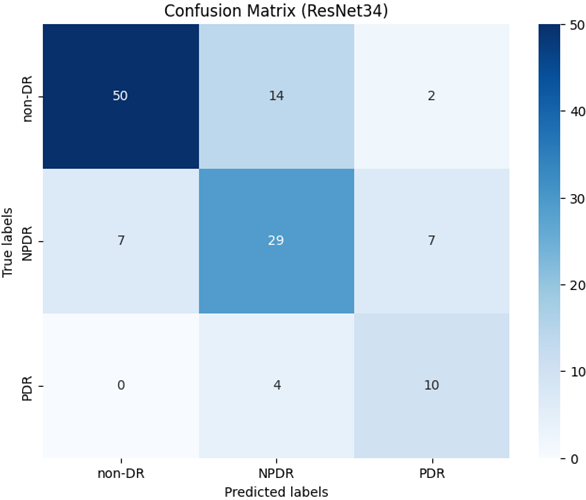
\includegraphics[draft=false, width=\textwidth]{gambar/confusionMatrixResnet34class-weighted_bestTrain.png} 
            \caption{Image D}
            \label{fig:2b}
        \end{minipage}
        \begin{minipage}[t]{0.475\textwidth} %
            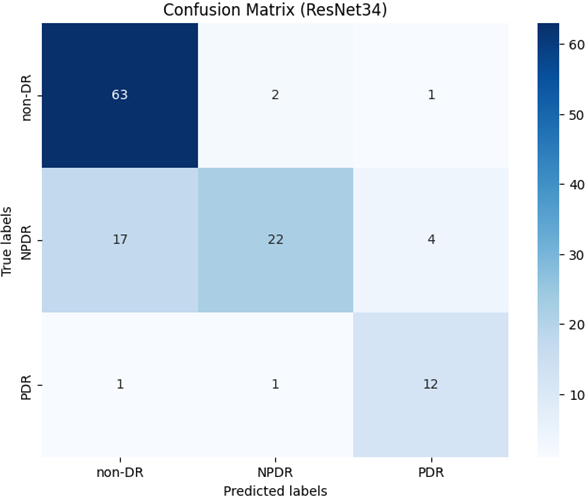
\includegraphics[draft=false, width=\textwidth]{gambar/confusionMatrixResnet34class-weighted_bestVal.png} 
            \caption{Image D}
            \label{fig:2b}
        \end{minipage}
        \begin{minipage}[t]{0.475\textwidth} %
            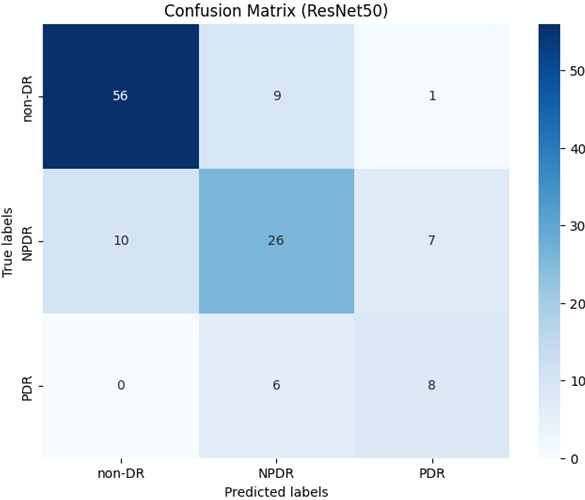
\includegraphics[draft=false, width=\textwidth]{gambar/confusionMatrixResnet50class-weighted_bestTrain.png} 
            \caption{Image D}
            \label{fig:2b}
        \end{minipage}
        \begin{minipage}[t]{0.475\textwidth} %
            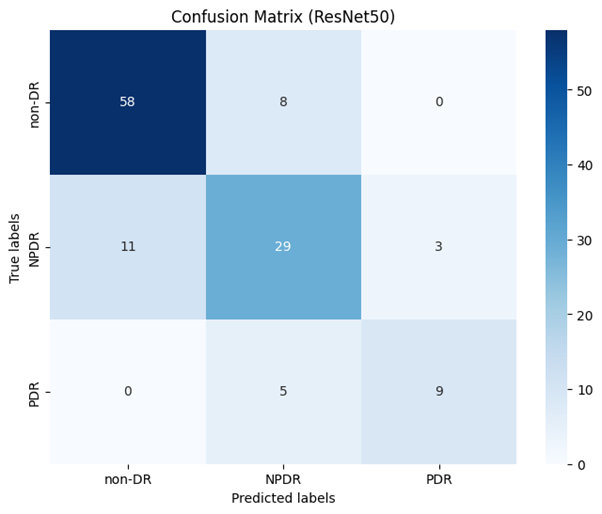
\includegraphics[draft=false, width=\textwidth]{gambar/confusionMatrixResnet50class-weighted_bestVal.png} 
            \caption{Image D}
            \label{fig:2b}
        \end{minipage}
        \begin{minipage}[t]{0.475\textwidth} %
            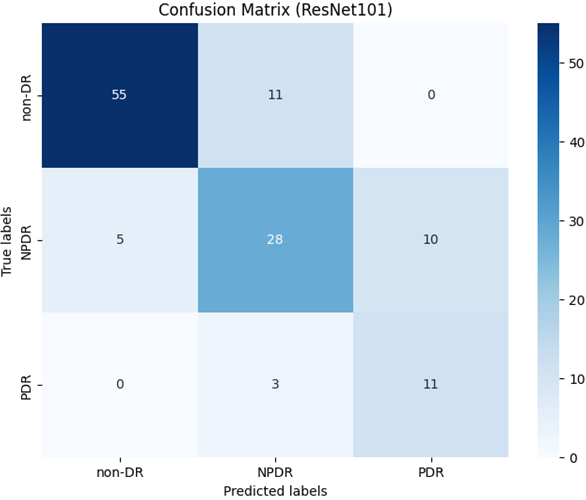
\includegraphics[draft=false, width=\textwidth]{gambar/confusionMatrixResnet101class-weighted_bestTrain.png} 
            \caption{Image D}
            \label{fig:2b}
        \end{minipage}
        \begin{minipage}[t]{0.475\textwidth} %
            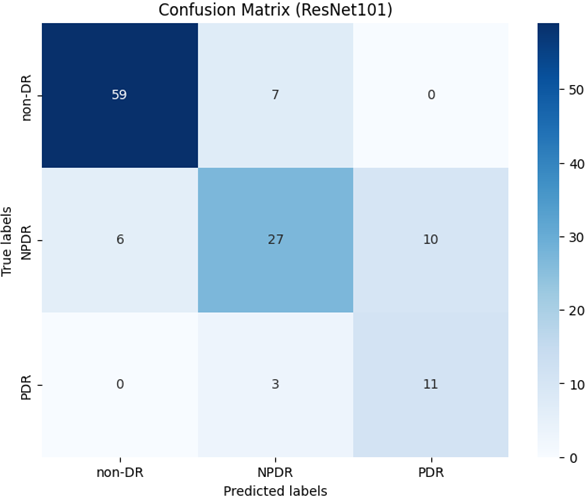
\includegraphics[draft=false, width=\textwidth]{gambar/confusionMatrixResnet101class-weighted_bestVal.png} 
            \caption{Image D}
            \label{fig:2b}
        \end{minipage}
        \caption{\emph{Confusion Matrix} dari model yang menggunakan penyesuaian \emph{class-weight}}
    \end{figure}

\subsection{Analisis Hasil}